\chapter{Atividade}

O objetivo do diagrama de atividade é focar nas ações, tarefas e fluxos de controle
em processos ou operações. O uso de um diagrama de atividade é uma prática essencial
na modelagem de processos e sistemas, proporcionando uma representação visual clara
do fluxo de controle das atividades. Suas principais características incluem a capacidade
de compreensão do funcionamento de um processo. Além disso, estes diagramas permitem
a análise e otimização de fluxos de trabalho, a identificação de ineficiências e a
comunicação eficaz entre equipes e partes interessadas. Com a capacidade de representar
responsabilidades, recursos e integração de sistemas, os diagramas de atividades
são uma ferramenta valiosa para o planejamento de projetos, documentação de processos
e aprimoramento da eficiência operacional em uma variedade de contextos, desde desenvolvimento
de software até gerenciamento de negócios e engenharia de sistemas.

Para ilustrar esse fluxo do cliente para cadastramento de uma nova rotina de um usuário
não identificado, considere o diagrama de atividade a seguir:

\begin{figure}[h]
  \centering
  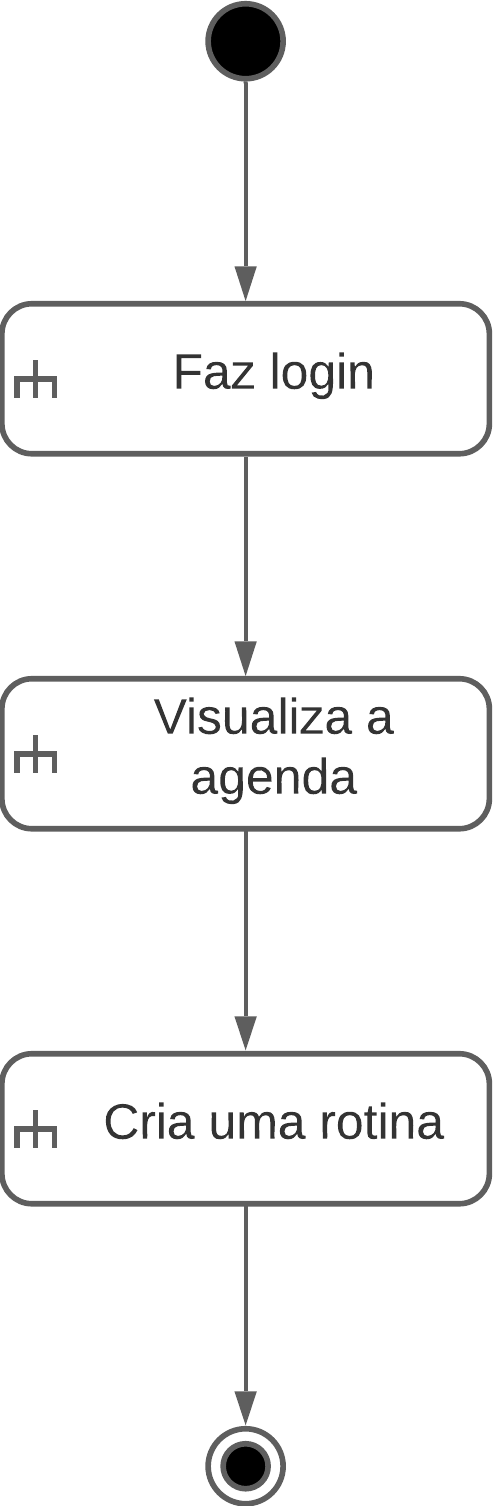
\includegraphics[scale=0.5]{images/diagrams/activity-one.png}
\end{figure}

\newpage
Esse diagrama de atividade visualiza o fluxo de forma clara, mostrando a sequência
de etapas e a lógica por trás do cadastramento de uma nova rotina. Cada ação é representada
por ícones de ação, e as setas conectam as atividades na ordem correta, garantindo
que o processo ocorra de maneira organizada e eficiente.

\begin{figure}[h]
  \centering
  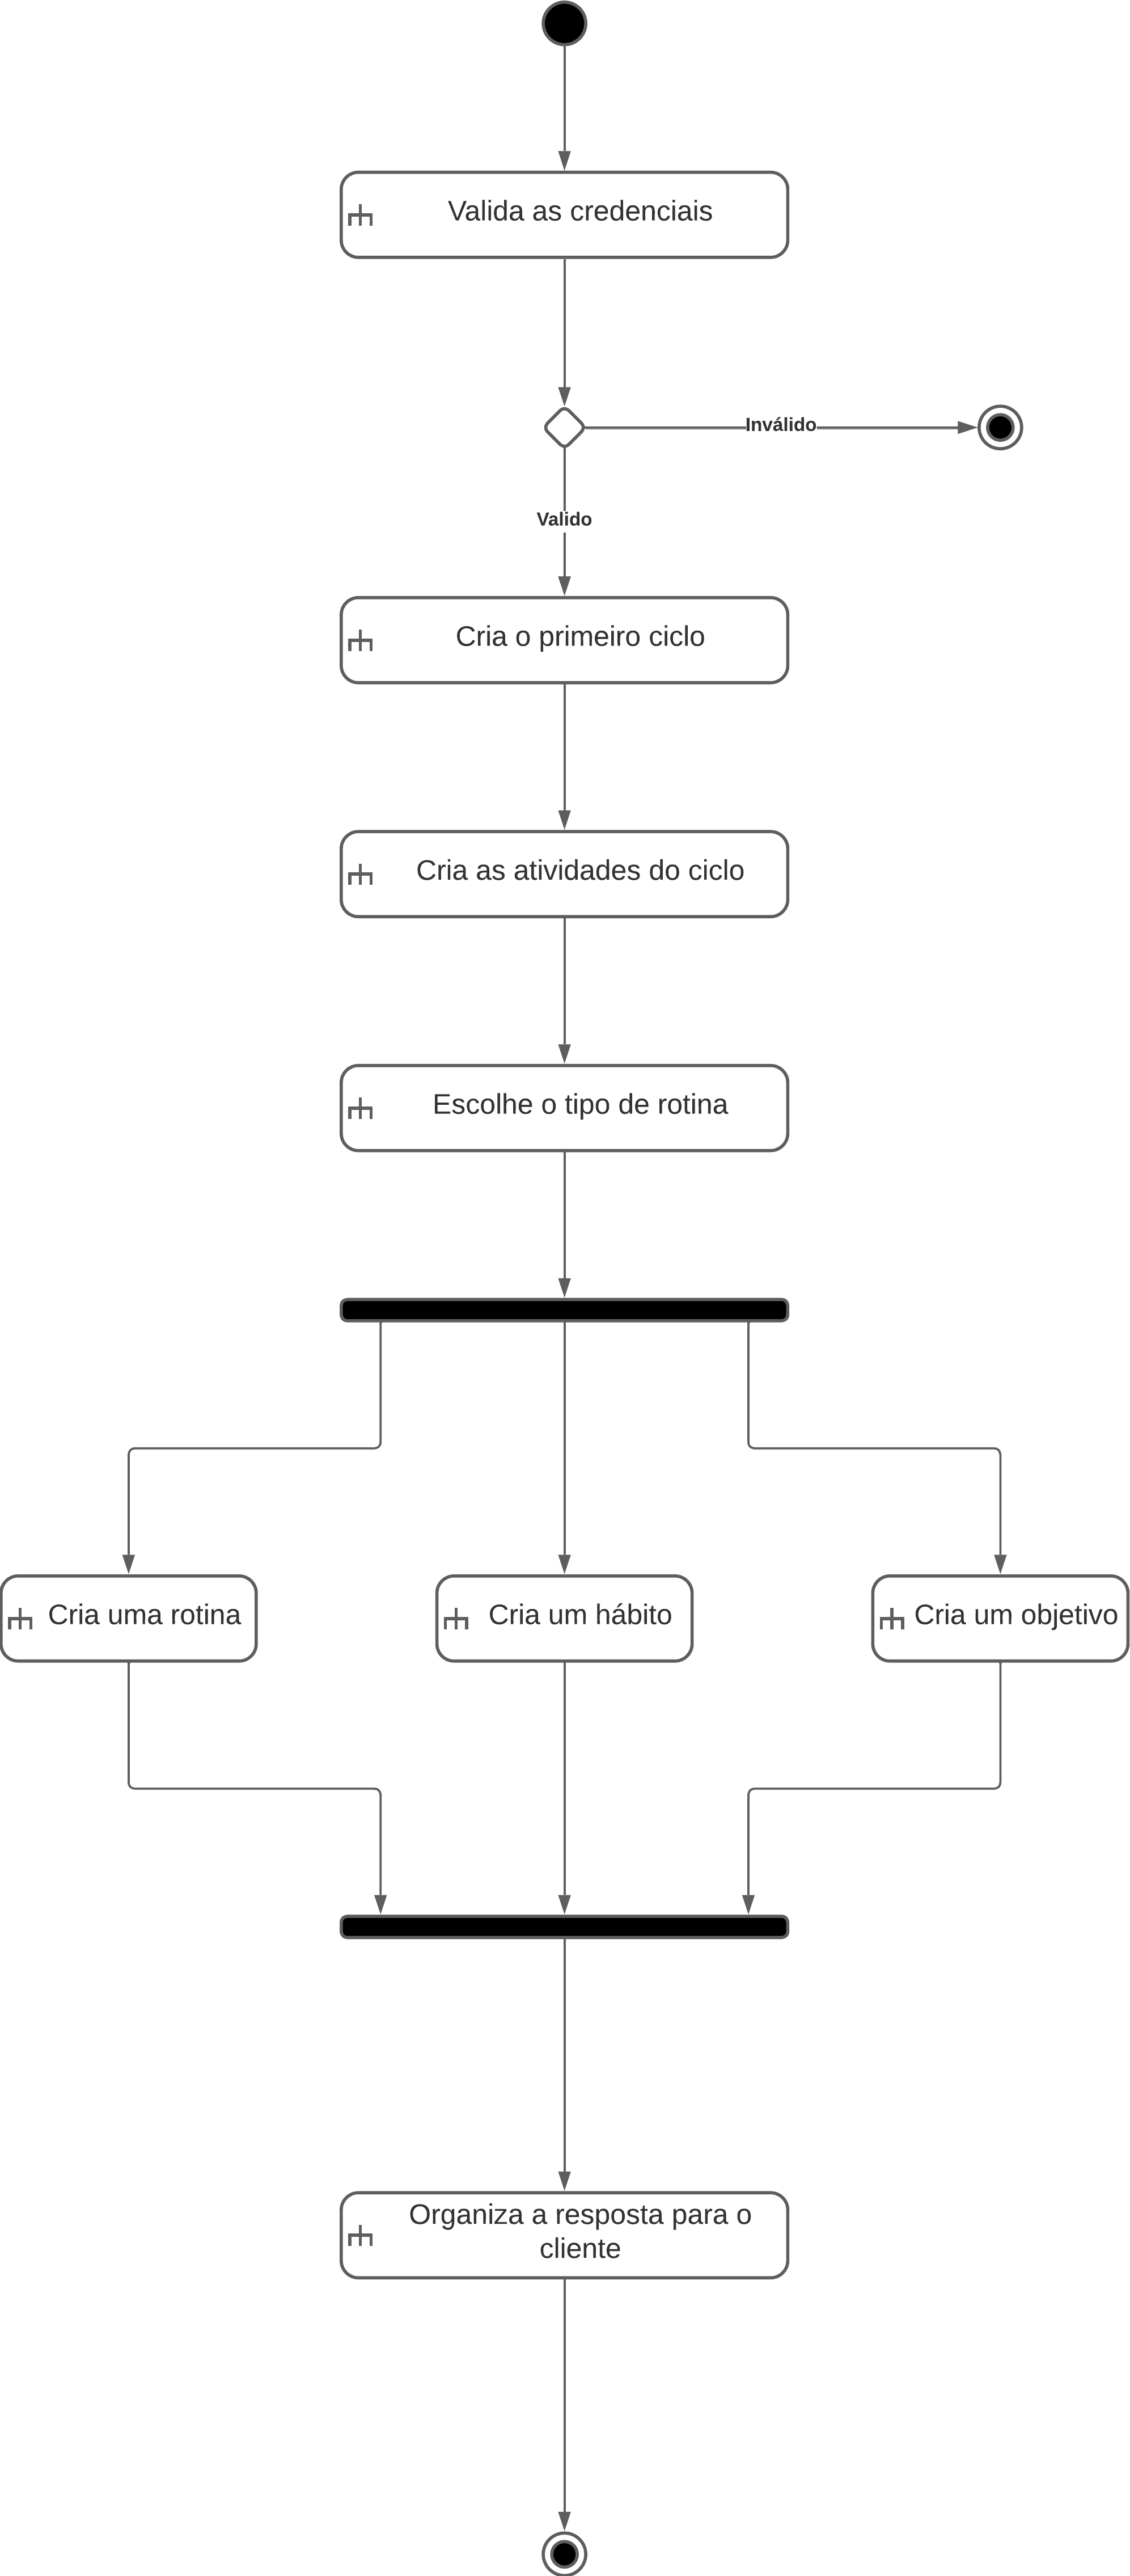
\includegraphics[scale=0.5]{images/diagrams/activity-two.png}
\end{figure}

\newpage
O processo de criação de uma nova rotina começa com a validação das credenciais obtidas
na etapa anterior. Caso inválido, o solicitante não consegue prosseguir com o fluxo.
Caso válido, é criado o primeiro ciclo e em seguida as suas atividades. Como uma
rotina pode ter diferentes tipos, com base nas informações fornecidas, é escolhido o tipo
sendo possível ser: rotina; hábito; ou objetivo. Para finalizar, as informações são
organizadas e entregues ao solicitante.
